\chapter{The Brain, The Computer and The Interface}

\epigraph{Deus ex machina!}{Aeschylus}

%\quotation{ \textit{...the brain is not a passive decoder of information but a dynamic and distributed modeler of a reality comprised of a multitude of feedback, local, modulatory, and feedforward neural pathways conjuring a vast and elaborate organic spatiotemporal grid \cite{nicolelis2011beyond}} } 

\vspace{10px}

%De 15 a 30 referencias

%La idea es sacar info del libro de bci el manual ultimo y del paper de wolpaw de nature.

%La relación entre la senial ruido obtenida en el experimento de LIGO y la que se obtiene en EEG.

With Vidal's work in 1970s, Brain-Computer Interfaces started as a technological amusement, and it steadely moved toward a mature and highly researched area of work.  Outstanding success has been achieved with invasive BCI, i.e. with surgically implanted electrodes. Success stories has been made public like Braingate's implant on Jan Scheuermann, Cathy Hutchinson and Dennis Degray \cite{Pandarinath2017}.  Other works include the total reproduction of arm movement \cite{c27}, the restoration of reaching and grasping movements through a brain-controlled muscle stimulation device on a person with tetraplegia \cite{Ajiboye2017} and the remote control of a manipulator by a macaque using brainwave information \cite{c29} albeit of persistent biocompatibilities issues and the pervasive complexity and risks of surgical procedures. One noteworthy aspect of this novel communication channel is the ability to transmit information from the Central Nervous System (CNS) to a computer device and from there use that information to control a wheelchair~\cite{Carlson2013}, as input to a speller application~\cite{Guger2009a}, in a Virtual Reality environment~\cite{Lotte2013} or as aiding tool in a rehabilitation procedure~\cite{Jure2016}.  Other novel applications include the real-time control of flight simulators \cite{Nourmohammadi2018} and the implementation of neuroadaptive interfaces where the computer detects the correctedness of a given command based on brainwave analysis \cite{Zander2016}.

Overall, the holly grail of BCI is to implement a new complete and alternative pathway to restore lost locomotion~\cite{WolpawJonathanR2012}.

\begin{chronology}[5]{1966}{2014}{90ex}[\textwidth]
\event{1966}{Kamiya, Neurofeedback for $\alpha$ waves}
\event{1969}{Fetz, Operand Conditioning}
\event{1973}{Vidal, first use of BCI word}
\event{1987}{Donchin \textbf{P300}}
\event{1989}{Hiraiwa, Bereitschaftspotentials}
\event{1991}{Wolpaw $\mu$ \textbf{Wadsworth BCI}}
\event{1993}{Pfurtscheller SMR \textbf{Graz BCI}}
\event{1995}{Jane Huggins invasive BrainGate}
\event{1997}{Anderson, Mental Tasks}
\event{1999}{Birmahuer SCP}
\event{2001}{Nicolelis, invasive BCI on primates}
\event{2003}{Middendorf, SSVEP}
\event{2006}{Millan, ErrP}
\event{2008}{Blankertz, adaptive \textbf{Berlin BCI}}
\event{2010}{Schalk, ECoG BCI}
\event{2012}{Zander, Passive BCI \textbf{pBCI}}
%\event{\decimaldate{25}{12}{2001}}{three}
\label{fig:story}
\end{chronology}

Figure \ref{fig:story} shows a brief chronology of the main events in BCI history, starting from the early works on Neurofeedback in the 70s and walking throught the different paradigms.  In recent years, this discipline has gained mainstream public awareness with worldwide challenge competitions like Cybathlon~\cite{Riener2014,cybathlon2} and even been broadcasted during the inauguration ceremony of the 2014 Soccer World Cup.  New developments are approaching the out-of-the-lab high-bar and they are starting to be used in real world environments~\cite{Guger2017,Huggins2016}.  Moreover, BCI research had rampantly been advanced accomplishing a BCI Society, a BCI Journal, BCI Award, annual conference meetings, practical applications, myriads of startups companies and even included in the Gartner list of Hype technologies \cite{GartnerHype2016}. 

From its root as assistive technology it has now expanded to include several application niches like Temporal induced disability, Neuroergonomy, early detection of human error, affective computing, biometric authentication, teleprescence (improvement of haptic interface), cyberinfrastructure and assistive robotics.  Intensive care units (ICU) and disorders of consciousness (DoC) \cite{Annen2018} (detection of remaining brain activity in comatose patients) are recent disciplines where BCI is showing tremendous prospects and possible applications.  

Their adoption as a clinical tool is still years ahead.  Stroke Rehabilitation is the only area where clinical trials for BCI are being conducted. It is understood that the neurofeedback provided by a BCI interface improves the prognosis of motor rehabilitation \cite{Ang2011}.

\vspace{10px}

\begin{story}[BCI Definition (circa 2018)]
\theoremstyle{definition}
\begin{definition}{}
\label{def:BCI}
\textit{A system that measures central nervous system (CNS) activity and converts it into artificial output that replaces, restores, enhances, supplements, or improves natural CNS output and thereby changes the ongoing interactions between the CNS and its external and internal environment \cite{WolpawJonathanR2012}.}
\end{definition}
\end{story}

Despite all this, its primary objective, its core motive of moving into real applications for disabled people has yet to come \cite{Brunner2014,Jeunet2014,Toward2013}. They still lack the necessary robustness, and its performance is well behind any other method of human computer interaction, including any kind of detection of residual muscular movement~\cite{Clerc}. Among the many and current challenges of BCI \cite{Brunner2014} one which is still perennial is precisely their inability to be used and applied outside the BNCI community and specifically in clinical context.  

%BCIs are currently in a plateau.  BCNI Horizon, what the people is saying.  OpenBCI and the Wearables movement.
% The convergence of invasive BCI and noninvasive BCI into a huge community and the appearance of myriad of comapnies that are exploring the technology.
Quoting experts in the field,

\vspace{10px}

\textit{"We yet have an impractical and inaccessible exotica for very specific user groups" (Allison 2010)\cite{Allison2010}}

\vspace{10px}

\textit{"Effectiveness of non-invasive BCI systems remain limited…" (Wolpaw 2011) \cite{Wolpaw and Wolpaw2011}}

\vspace{10px}

\textit{"…to ponder if BCIs are really promising and helpful, or if they are simple a passing rod, reinforced by their sci-fi side..." (Lotte 2016)\cite{Lotte2016}}

\vspace{10px}

The feasibility of the system has been proved but there are several challenges in BCI that need to be tackled. They can be summarizing as 
increasing the ITR, the pervasive low signal-to-noise ratio of brainwaves, particularly of noninvasive signals \cite{Lotte2018}, the reliability of the system, its portability, and the usability of the system \cite{Wang2018}, and at the same time decreasing the setup, the training and,calibration time and the subject's inter/intra variability. The search for practical, relevant, and invariant \textit{features} that convey good-enough information about the underlying cognitive process is still a goal to be achieved \cite{Perdikis2014}.  Ethical aspects of BCI \cite{Yuste2017} must also be considered and handled: cybersecurity threats and privacy concerns,  agency and identity issues that might be occurring by deleterious plasticity with BCI users and the strict peg to the \textit{Primun non vocere}~\footnote{\textit{First, do not harm}, in reference to the Hippocratic Oath} mandate.


\section{Brain Computer Interface Model and Architecture}

The draft architecture of a BCI system can be summarized in Fig \ref{fig:bciblockdiagram}.  A volitional control, a will to transmit information, is exerted by a user. A brain imaging device captures his/her signals using a measurement modality.  A signal acquisition module obtains the brainwaves and the information is digitalized and transmited to a computer device.  Signal preprocessing is applied to eliminate nuisances and artifacts and to enhance the Signal to Noise Ratio (SNR), or to apply spatial or frequency filters.  In the next step, a \textit{feature} is carefully constructed in order to differentiate at least between two different mental states.  Finally a classification step is applied to derive the actual information bit out of the system.   An Application System uses this information to affect some external device.  By visual or any other sensory means, the feedback is fed back to the user and a loop is finally closed.

The central point of this system is called the \textit{Brain Machine Dilemma} \cite{WolpawJonathanR2012}.  The underlying idea is that the BCI system adapts to the user's thinking patterns but at the same time the brain is adapting to what the system is doing, and changing their own signals in the process.  This is the reason why it is often called, a \textit{co-adaptive system}, where two different intelligent devices, one biological and the other electronic, try to adapt to each other.

\begin{figure}[]
\centering
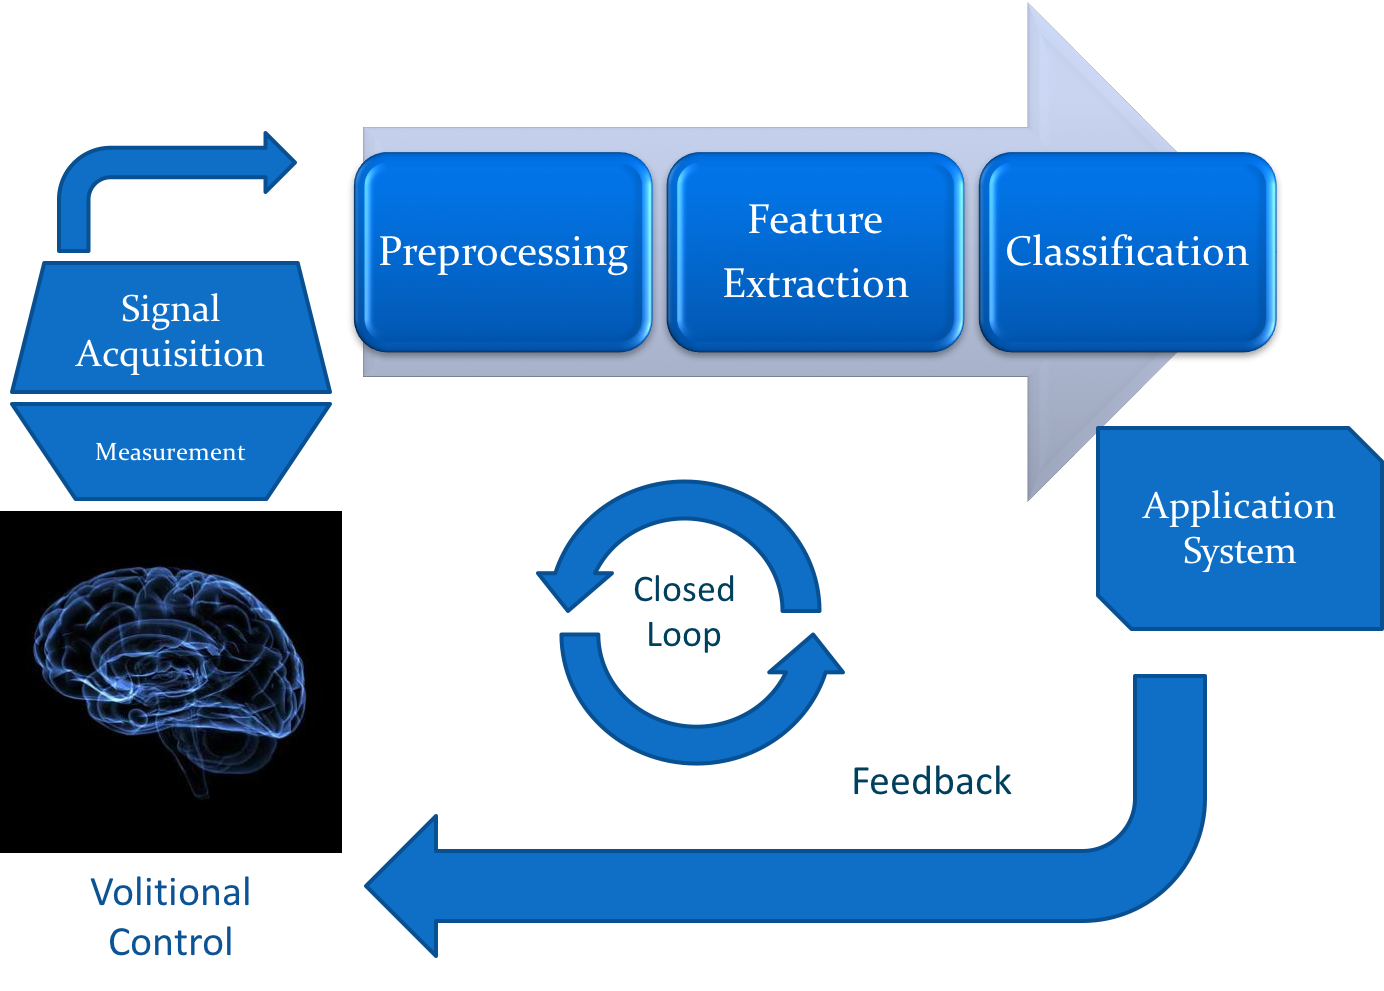
\includegraphics[scale=0.5]{images/bcichart.png}
\caption[BCI Block Diagram]{General components of a BCI system.}
\label{fig:bciblockdiagram}
\end{figure}

The basic model of any BCI is to take a multichannel digital signal $\mathbf{x}(n)$, and transform it to an output control signal $y(n)$ which can be a scalar or binary function.  The BCI system can be modeled as the transformation $T$.

\begin{equation}
y(n) = T\left[\mathbf{x}(n)\right]
\label{eq:bcimodel}
\end{equation}

What a BCI system must do, is to take at least a single bit of information out of $y(n)$ and use that information to derive some action. 

\section{Signal Processing}

From this signal processing point of view, BCIs are:

\begin{itemize}
\item Causal:  $ y(n) = f( \mathbf{v}(m) ) $, where $ m \leq n $.  The action of a BCI system depends on the history of the captured brainwaves.
\item Dynamic: $ y(n) = f( \mathbf{v}(m),  \mathbf{\dot{v}}(m),\mathbf{\ddot{v}}(m),...) $.  A BCI system is dynamic, where the output function do not depend only on the current value being observed, it does depend on its dynamic interactions.
\item Time invariant: $ y(n) = T\left[ \mathbf{v}(n) \right] \Rightarrow y(n-k) = T\left[ \mathbf{v}(n-k) \right] $.  The output of a BCI system does not depend on the particular time frame where it is being used.  However, Adaptive BCI, which do adapt to the user behavior are in general time variant.
\item Nonlinear: a system is linear when $T\left[ a_1 \mathbf{v}(n) + a_2 \mathbf{v}(n) \right]  = a_1 T \left[ \mathbf{v}(n) \right] + a_2 T \left[ \mathbf{v}(n) \right] $. Due to brainwave complexity, BCI systems are not linear.
\item Multirate or broadband \cite{Miller2010}:  The energy of brainwave spectrum is not confined to a certain band, and almost all frequency channels convey some information.
\end{itemize}

There are several filters that can be applied to the system to eliminate artifacts, enhance the signal, and to ease the detection of the discriminative information.

\textbf{Static Filters} like square or logartihmic were traditionally used in analog signal processing and are currently already embedded in the measuring device.  Wiener and Kallman Filters are usually applied to invasive techniques~\cite{NeuralEngineeringBookBinHe}.  The filter, particularly when it is linear, can be viewed as the matrix $M$ in:

\begin{equation}
y(n) = M T\left[\mathbf{x}(n)\right]
\label{eq:filters}
\end{equation}

\textbf{Spatial filters} are carefully adapted to the arrangement of sensors around or within the head and they emphasize the spatial structure of the information that is being captured. Derived from neuroscience research, locations on the head are structured according to neuroanatomical planes or axes and normally the brain, or the head, are divided in different anatomical regions (Figure \ref{fig:neuroanatomy}).   

\textbf{Spectral Filters}, on the other hand, do consider brainwaves as another digital signal, and they perform different transformations based on the spectral information contained within the signal $\mathbf{x}(n)$.  They can be combined and aggregated creating  \textit{Filter Banks} to enhance signal quality. 


\begin{figure}[htb]
\centering
\subfigure[Neuronal Planes]{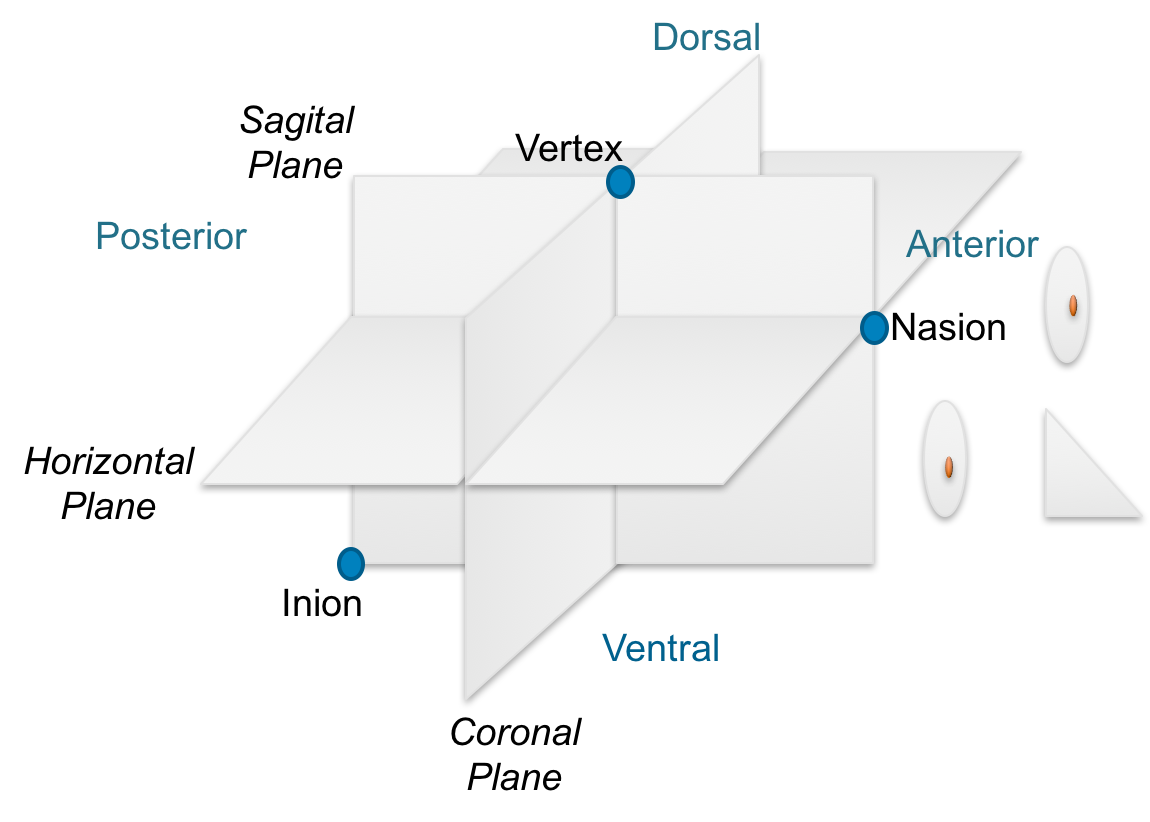
\includegraphics[scale=0.4]{images/neuralplanes.png}}
\subfigure[Neuroanatomical regions of the brain.]{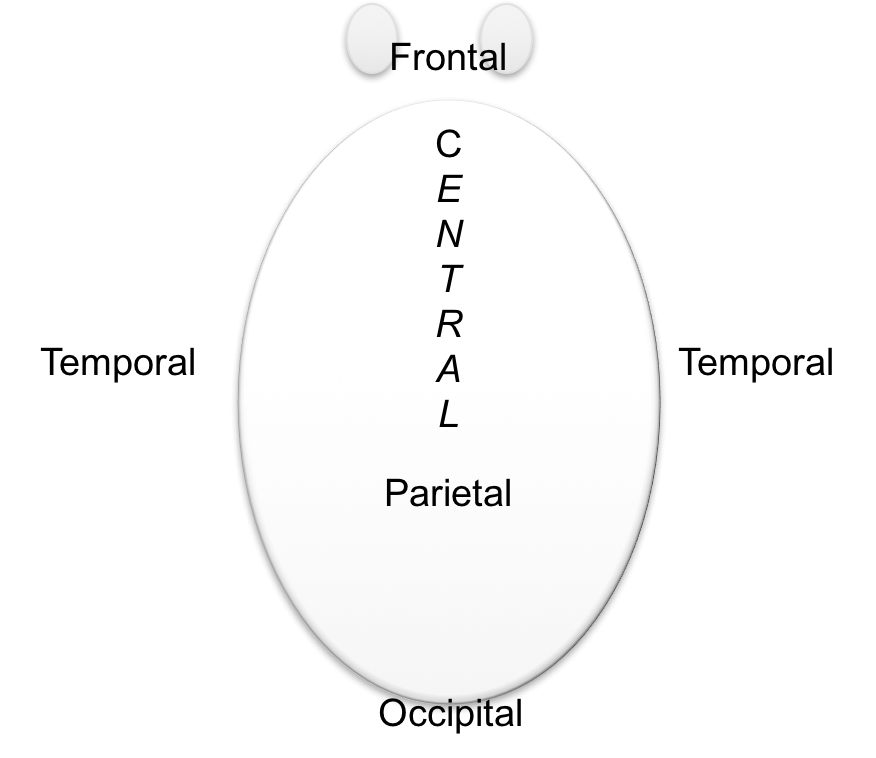
\includegraphics[scale=0.4]{images/neuroanatomy.png}}
\caption[Neuroanatomical structures of the brain]{Neuronal Planes regularly used in neuroscience research.  In BCI they are used to understand electrode location and spatial filters.}
\label{fig:neuroanatomy}
\end{figure}

%\begin{figure}[]
%\centering
%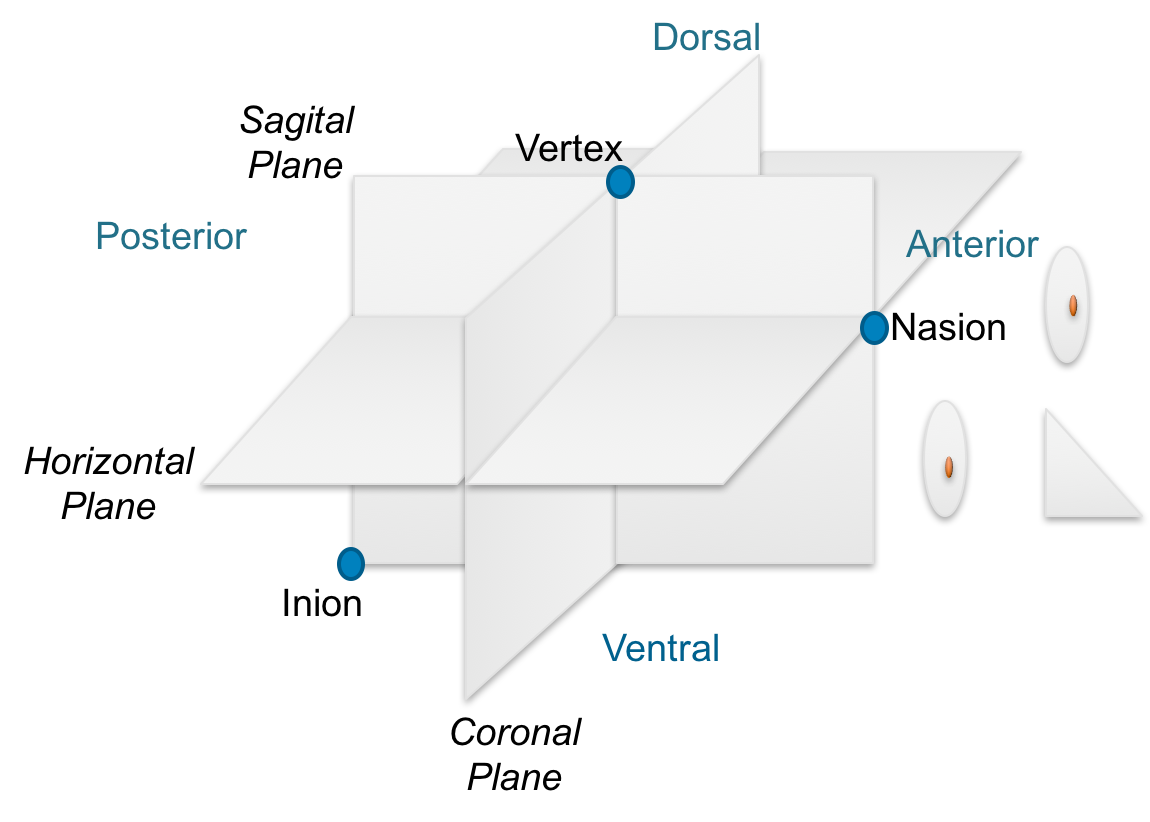
\includegraphics[scale=0.5]{images/neuralplanes.png}
%\caption[Neural Planes]{Neuronal Planes regularly used in neuroscience research.  In BCI they are used to understand electrode location and spatial filters.}
%\label{fig:neuralplanes}
%\end{figure}
%
%\begin{figure}[]
%\centering
%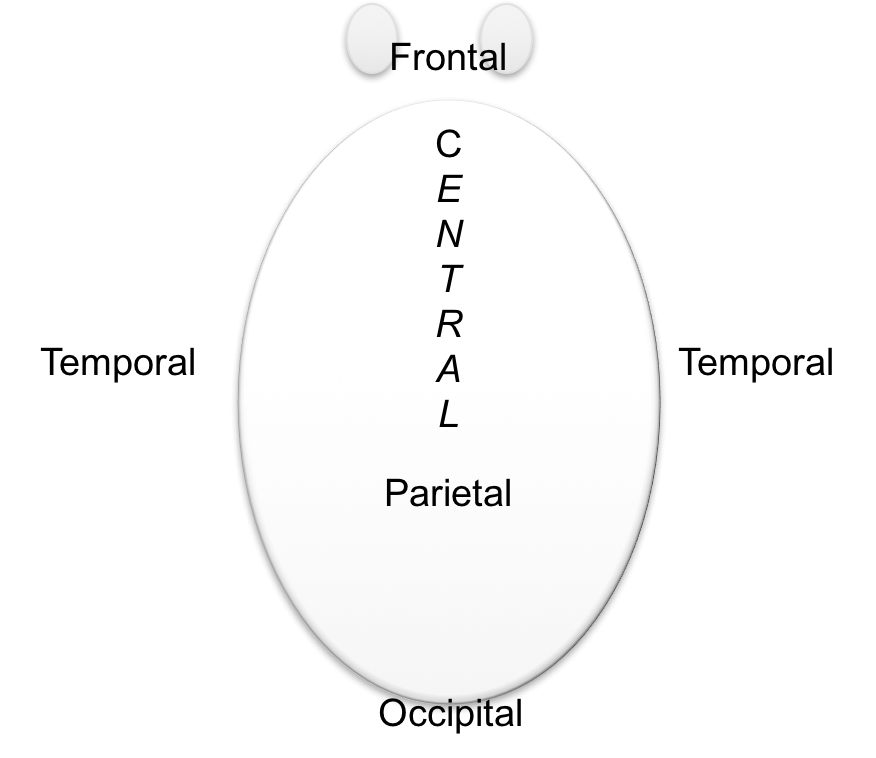
\includegraphics[scale=0.5]{images/neuroanatomy.png}
%\caption[Neuroanatomy]{Neuroanatomical regions of the brain.}
%\label{fig:neuroanatomy}
%\end{figure}

\section{The Forward and Inverse Model}

Brainwaves are obtained via sensors, where each one of them captures only a part or a version of the information.  However, whatever is actually happening inside the brain can be only recovered indirectly from the \textit{Sensor Space}. From there, the information can be traced back to the real landscape where the information source is located, inside the \textit{Source Space}.  This is a regular problem found in Engineering and it is not different in BCI.  \textit{Calculating} the signal on each a sensor from a projection of a known source of information from within the head is called \textit{The Forward Problem}\cite{Parra2008,WolpawJonathanR2012}  and doing the opposite, \textit{estimating} the contributions of different sources to whatever activity is found on sensors is called  \textit{The Inverse Problem} .  The latter is more relevant in BCI because it allows to determine source origins that can be mapped more directly to cognitive activities.  However, this kind of problem is highly ill-posed and it is precisely where the majority of the efforts of this discipline are concentrated due to its complexity.

Particularly for noninvasive electrophysiological modalities, an additional problem makes thing harder.  Due to its electromagnetic properties, the brain acts like conductive gel, and any signal that is generated inside the brain is irradiated to every direction and it can influence every sensor regardless of its position.  This is called \textit{Volume conduction} \cite{Nam2018} and can be visualized in Figure~\ref{fig:volconduction}.

\begin{figure}[]
\centering
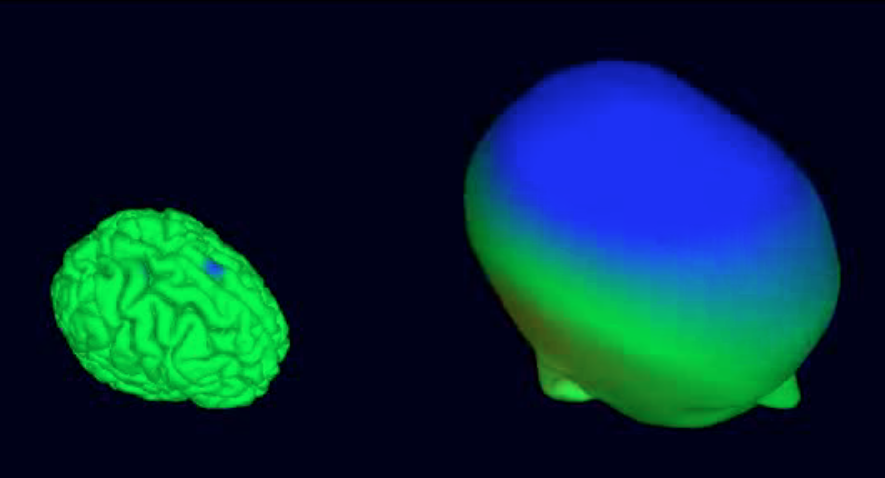
\includegraphics[height=6cm,width=14cm]{images/volconduction1.png}
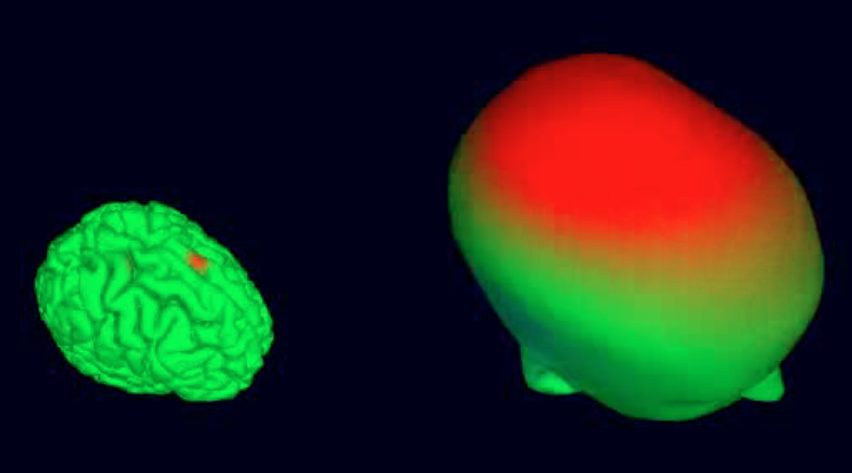
\includegraphics[height=6cm,width=14cm]{images/volconduction2.png}
\caption[EEG Volume Conduction]{A source signal with positive/negative polarity is generated in a very specific region of the brain but due to volume conduction their influence affects a widespread area of the scalp where sensors are located (Image from Swartz Center for Computational Neuroscience) }
\label{fig:volconduction}
\end{figure}

\section{Brain Imaging Technologies}

The measuring technique determines the most important taxonomic differentiation in BCI, according to how they extract the information from the CNS Central Nervous System.

\begin{enumerate}
\item fNIRS: functional Near Infra Red Spectroscopy.
\item EEG: Electroencephalography
\item MEG: Magnetoencephalography
\item PET: Positron Emission Tomography
\item fMRI: functional Magnetic Resonance Imaging
\item ECoG: Electrocorticography 
\item INR: Intracortical Neuron Recordings.  Particularly LFP and microelectrodes (Utah array).
\end{enumerate}

ECoG and INR are invasive technologies that require some neurosurgery and an implantation of electrodes inside the skull the former, and inside the brain the latter.  All the remaining imaging techniques are external or noninvasive.  Hybrid BCI, or Brain Neural Computer Interface, are BCI devices that use not only signals from the CNS, they utilize any kind of available biosignal that can be volitionally modulated to transmit information (this is called dependant BCI).  On the other hand, when the pace of the BCI is regulated by external stimulus it is called synchronous and when the user choose their own pace to transmit information, it is often called asynchronous or self-paced BCI.

Recent years have seen an incredible advance of Passive BCI, pBCI \cite{Zander2010}.  The original definition of BCI did not include Passive modalities but per definition \ref{def:BCI} it is now part of this discipline.  The important aspect is that passive technologies do not entail necessary the volitional requirement to transmit information.  EEG-based passive BCI is a promising and advancing area of research and of commercial applications.

\section{Electroencephalography}

Above all, Electroencephalography (EEG), is the most widespread method to gather information from the CNS in a non-invasive way. They are of particular interest in BCI mainly because of their non-invasiveness, their optimal time resolution and acceptable spatial resolution. Moreover, they are portable, cheap, wearable and can be more easily integrated into fashionable designs aimed for real users, which prefer cap-like devices~\cite{Huggins2015}. 

The Electroencephalography consists on the measurement of small variations of electrical currents over the scalp.  This represents the summed activity of post-synaptic potentials PSPs of pyramidal neurons located perpendicular to the scalp~\cite{Nam2018}. Only one percent of synchronized activity of pyramidal neurons are stronger that the remaining desynchronized neurons~\cite{Nunez} and explain ninety-nine percent of the signals obtained from EEG.  This brain imaging technology is one of the most widespread used methods to capture brain signals and was initially developed by Hans Berger in 1924 and has been extensively used for decades to diagnose neural diseases and other medical conditions.

%Routinely physicians explore morphologically these raw EEG signals scavenging for signs of disease or irregular patterns and they have been doing this since almost the dawn of the technology at the hands of Hans Berger. Sleep spindles, Lambda waves, K-Complexes, Vertex waves, Positive Occipital Sharp Transients and more visual features had been identified with relevant clinical characterizations [16]. Even within the BCI community, visually extracting artifacts for offline processing is a common and well known practice [1,11]. 

%The EEG signal goes from 10-100 microvolts
%monopolar, reference, averaged, 
%bipolar
%segmentation is commong, which is generally called epoching
%trials are general realizations of the experiment.
%tampering window could be gaussian, hamming, blackman, hanning
%Impedance

The first characterization that Dr. Berger detected was the Visual Cortical Alpha Wave, the \textit{Berger Rythm} \cite{Jansen1991}.  He understood that the amplitude and shape of this rhythm was coherently associated to a cognitive action (eyes closing).  
We should ask ourselves if the research advancement that came after that discovery would have happened if it weren't so evident that the shape alteration was due to a very simple and verifiable cognitive process.

The EEG signal is a highly complex multi-channel time-series.  It can be modeled as a linear stochastic process with great similarities to noise \cite{Thakor2004}.  It is measured in microvolts, and those slightly variations are contaminated with heavy endogenous artifacts and exogenous spurious signals.  
 
\begin{figure}[]
\centering
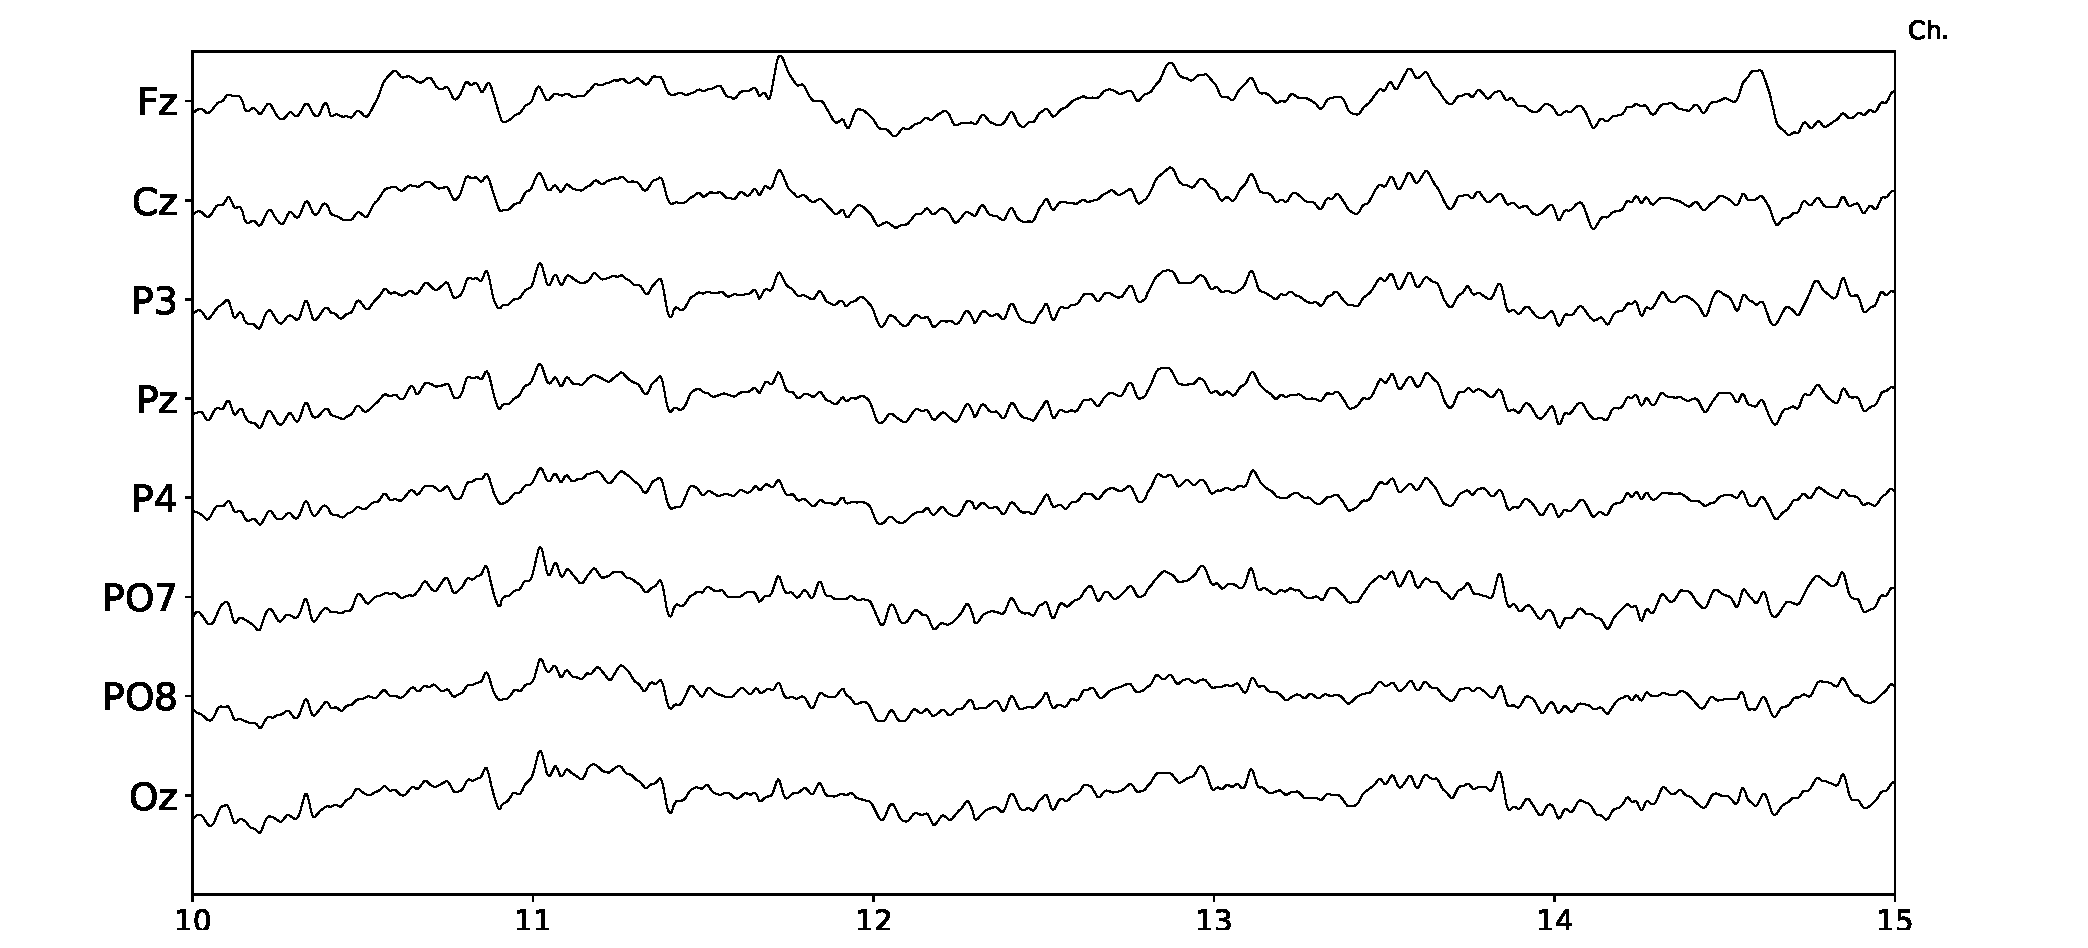
\includegraphics[height=6cm,width=14cm]{images/sampleeeg.eps}
\caption{Sample EEG signal obtained from (g.Nautilus, g.Tec, Austria). Time axis is in seconds and five seconds are displayed.  The eight channels provided by this device are shown.}
\label{fig:sampleeeg}
\end{figure}


\begin{figure}[]
\centering
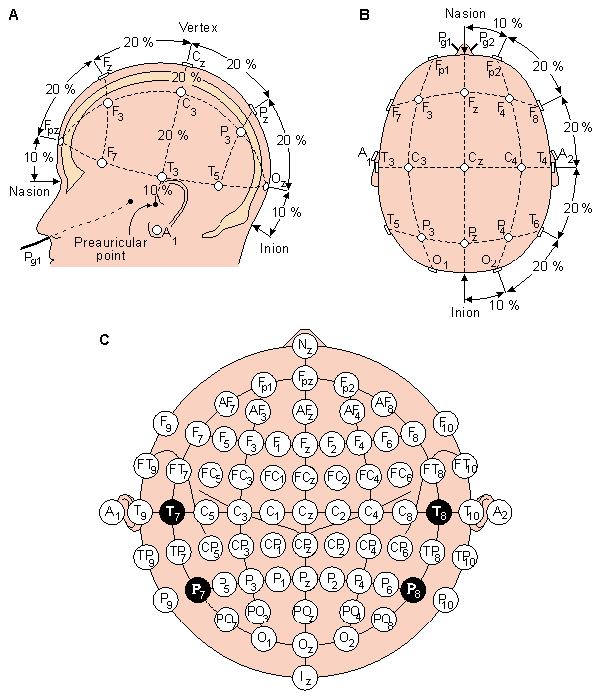
\includegraphics[height=6cm,width=6cm]{images/ElectrodePositions1020.png}
\caption[Electrode Locations]{International 10-20 system that standardize electrode locations over the scalp.}
\label{fig:electrodelocations}
\end{figure}

%locations.eps

The device that captures these small variations in current potentials over the scalp is called the Electroencephalograph (Figure \ref{fig:digitalelectroencephalograph}).  Electrodes are located in predetermined positions over the head, usually embedded in saline solutions to facilitate the electrophysiological interface and are connected to a differential amplifier with a high gain which allowed the measurement of tiny signals. Although initially analog devices were developed and used, nowadays digital versions connected directly to a computer are pervasive.  A detailed explanation on the particularities and modeling of EEG can be obtained from \cite{Jackson2014}, and a description of its electrophysiological aspects from \cite{Haberman2012}.

\begin{figure}[]
\centering
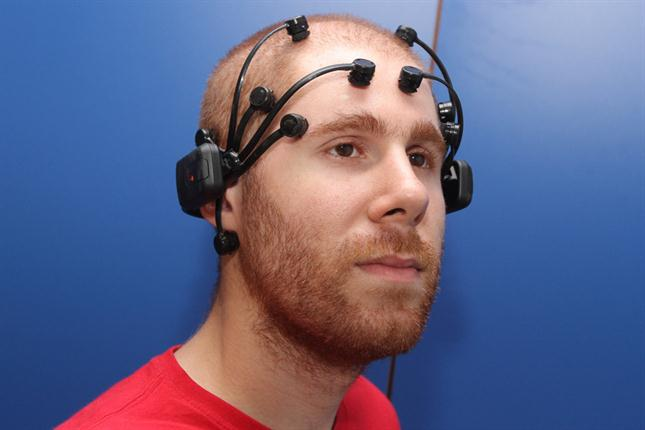
\includegraphics[height=4cm,width=7cm]{images/emotivsubject.jpg}
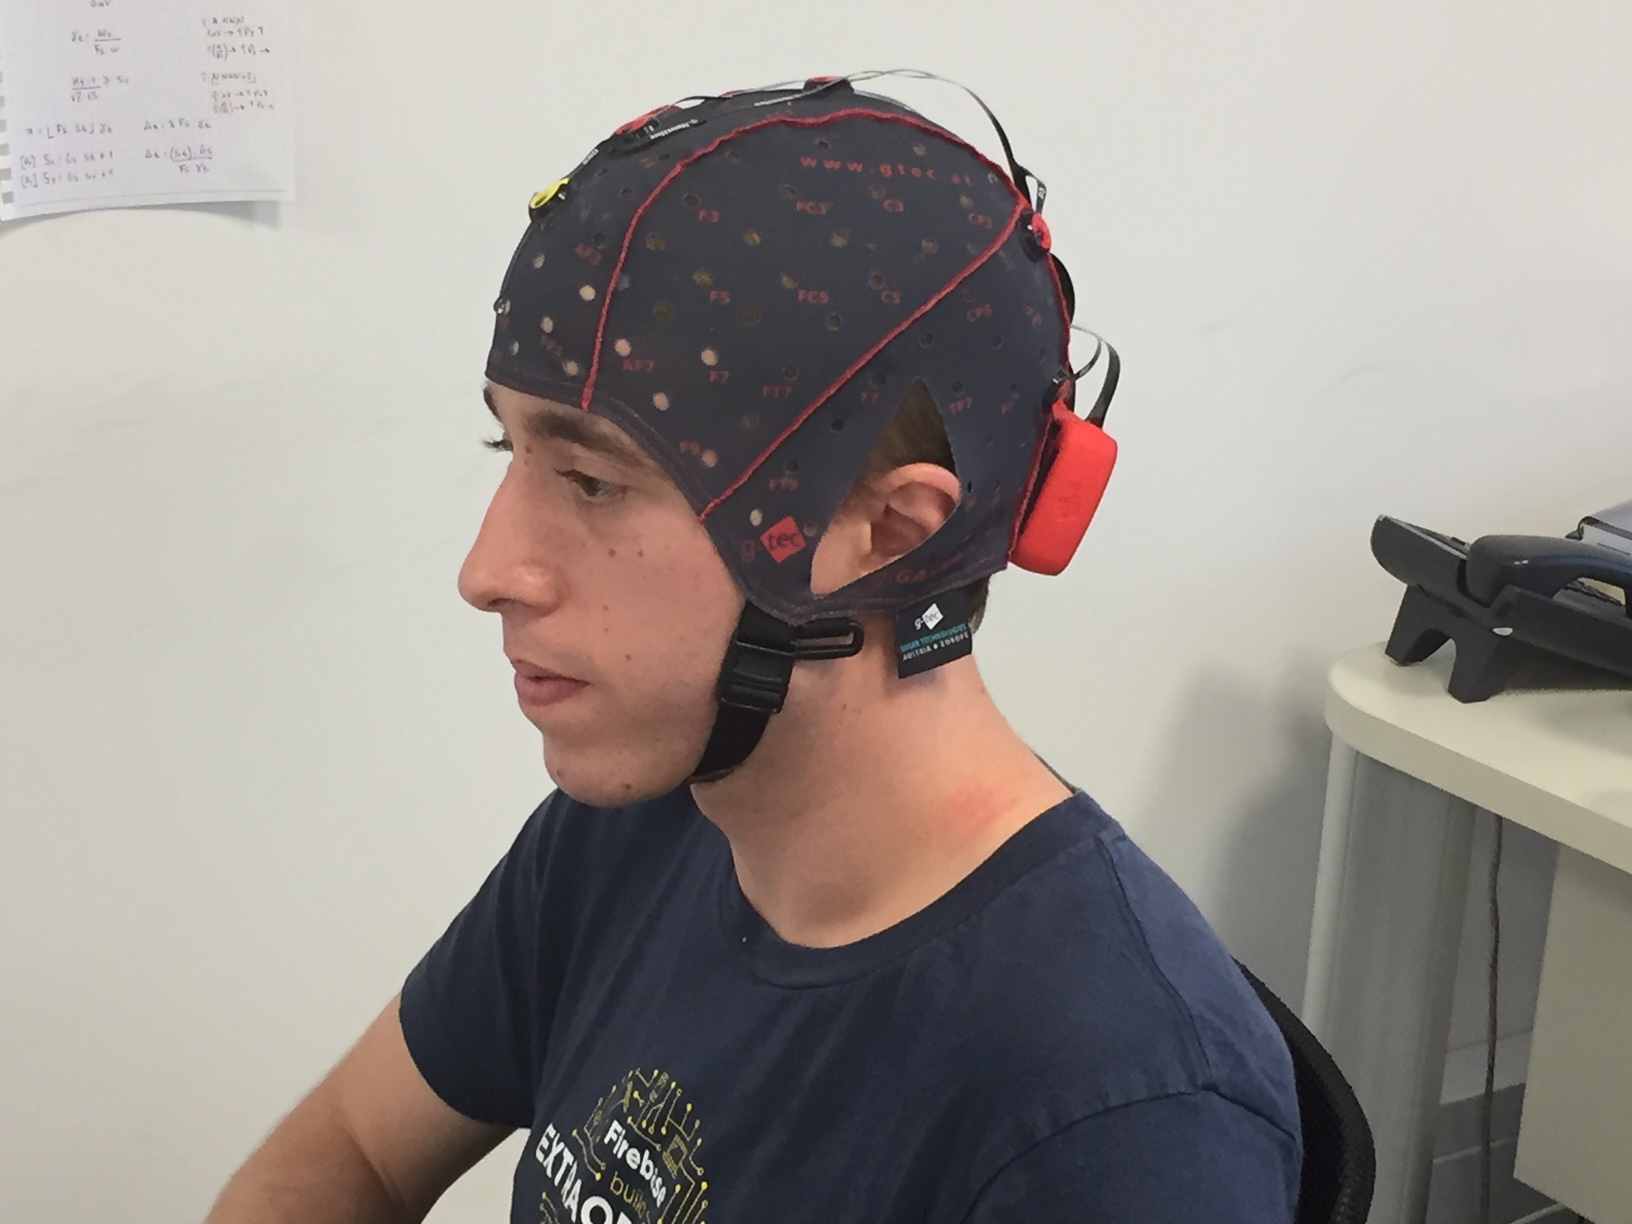
\includegraphics[height=4cm,width=7cm]{images/gTecsubject.jpg}
\caption[Wearable portable Digital Electroencephalograph]{Consumer-grade digital electroencephalograph.}
\label{fig:digitalelectroencephalograph}
\end{figure}


Overall, EEG signals can be described by their phase, amplitude,  frequency and \textit{waveform}.  The following components regularly  characterize EEG signals:

\begin{itemize}
\item Artifacts:  These are signal sources which are not generated from the CNS, but can be detected from the EEG signal.  They are called endogeneous or physiological when they are generated from a biological source like muscles, ocular movements, etc., and exogeneous or non-physiological when they have an external electromagnetic source like line induced currents or electromagnetic noise\cite{Weeda2012}.  Ambulatory studies or out-of-the lab studies introduces artifacts that are derived from the person movement from the FES and also from other devices in hybrid BCI, or multi-modal BCIs.
\item Non-Stationarity: the statistical parameters that describe the EEG as a random process are not conserved through time, i.e. its mean and variance, and any other higher-order moments are not time-invariant \cite{Jansen1991}.
\item DC drift and trending: in EEG jargon, which is derived from concepts of electrical amplifiers theory, Direct Current (DC) refers to very low frequency components of the EEG signal which varies around a common center, usually the zero value.  DC drift means that this center value drifts in time.  Although sometimes considered as a nuisance that needs to get rid of, it is known that very important cognitive phenomena like Slow Cortical Potentials or Slow Activity Transients in infants do affect the drift and can be used to understand some particular brain functioning \cite{Schomer2010}.
\item Basal EEG activity: the EEG is the compound summation of myriads of electrical sources from the CNS.  These sources generate a baseline EEG which shows continuous activity with a small or null relation with any concurrent cognitive activity or task.
\item Inter-subject and intra-subject variability: EEG can be affected by the person's behavior like sleep hygiene, caffeine intake, smoking habit or alcohol intake previously to the signal measuring procedure \cite{Farzan2017}.
\end{itemize}

Regarding how the EEG activity can be related to an external stimulus that is affecting the subject, it can be considered as

\begin{itemize}
\item Spontaneous: generally treated as noise or basal EEG.
\item Evoked: activity that can be detected synchronously after some specific amount of time after the onset of the stimulus.  This is usually referred as time-locked.  In contrast to the previous one, it is often called Induced activity.
\end{itemize}

\noindent Additionally, according to the existence of a repeated rhythm, the EEG activity can be understood as

\begin{itemize}
\item Rhythmic: EEG activity consisting in waves of approximately constant frequency.  It is often abbreviated RA (regular rythmic activity). They are loosely classified by their frequencies, and their naming convention was derived from the original naming used by Hans Berger himself:

\begin{itemize}
\item Alpha Waves (10 Hz)
\item Delta (0-4 Hz)
\item Theta (4-8 Hz)
\item Sigma (12-16 Hz)
\item Beta (12-30 Hz)
\item Gamma (30-100 Hz)
\item Omega (60-120 Hz)
\item Rho (250 Hz) hippocampal
\item Sigma Thalamocortical burst (600 Hz)
\end{itemize}

\item Arrhythmic: EEG activity in which no stable rhythms are present.  
\item Dysrhythmic: Rhythms and/or patterns of EEG activity that characteristically appear in patient groups and rarely seen in healthy subjects.
\end{itemize}

The number of electrodes and their positions over the scalp determines a Spatial Structure: signal elements can be generalized, focal or lateralized, depending on in which channel (i.e. electrode) they are found.

%Finally, indexes can be derived as  CFC, Cross Frequency Coupling,  Phase-Amplitude Coupling, Phase-Phase Coupling.


\section{BCI EEG Paradigms}

%Due to their popularity ($71.2\%$ of the BCI projects submitted to BCI Award 2016 were with EEG) BCI based on EEG are 

\textit{BCI Paradigms} are referred to noninvasive EEG-based BCI configurations that can be used to transmit volitional information.  The popularity of EEG ($71.2\%$ of the BCI projects submitted to BCI Award 2016 were with EEG)~\cite{GugerBook2016} pushed the adoption of paradigms exclusively for noninvasive BCI.   Their chronology can be found in Figure \ref{fig:story}. They are

\begin{enumerate}
\item Steady State Visual Evoked Potentials
\item Bereitschaftspotentials, Readiness Potential or Movement-Related Potentials
\item Motor Imagery
\item ERD/ERS: Event Related
\item Wadsworth BCI
\item Graz BCI
\item Selective Attention
\item P300
\item N400
\item Mental Tasks
\item Operant Conditioning
\item Slow Cortical Potentials
\item Berlin BCI



\end{enumerate}


\section{State of the Art of BCI Algorithms for EEG processing}

According to general layout of any BCI, Figure \ref{fig:bciblockdiagram}, specific algorithms or techniques are derived for both the Feature extraction and classification step.

The most relevant features used in BCI are:

\begin{itemize}
\item Time points:  the sequence of time series, often, concatenated in time or space.
\item Band Power: frequency based features.
\item Complexity:  based on complexity measurements like entropy, fractal.
\item Statistical: AR parameters, covariances matrix.
\end{itemize}

The most successfull used and verified classification methods for BCI \cite{Lotte2007} can be described as linear versions of popular Machine Learning tools.  Particularly, Support Vector Machines SVM, Linear Discriminant Analysis LDA and its variant SWLDA.  This one was also relevant for two reasons:  the first is that the stepwise identification of features improves the selection criteria and also the spatial filter that this procedure encompass.  Additionally, and more from a more pragmatic perspective, this method was included in the popular BCI2000~\cite{bci2000} package and was the default option for anyone doing ERP identification.  Spatial Filters have also being incorporated and have shown substantial improvement in classification accuracies.  The now classical Common Spatial Patterns CSP for the identification of Motor Imagery as well as the xDAWN algorithm for P300 identification.

Recent years (circa 2018) have seen the evolution of the methodology but the focus was not centered on any particular classification algorithm.  Instead how they are used became much more important~\cite{Lotte2018}.

\begin{itemize}
\item Ensemble Classifiers: SVM ensembles~\cite{Rakotomamonjy2008} and variants of Random Forest~\cite{Steryl2014}.  Features are segmented and divided and the forest performs a classification step on each part and maximizes classification accuracies.
\item Cross-Paradigm BCI: the use of Reinforced Signal RS with ErrP feedback or the use of SSVEP in combination with P300 detection~\cite{aca}.
\item Adaptive Classifiers: the parameters of the classifiers are adapted continuously and online adapting to the natural variation of the EEG signals~\cite{Lotte2018}.
\item Transfer Learning: transfer the calibration information obtained by users to new subjects.  This aims to eases the issue of the intra-subject variability in BCI .
\item RGC: Rienmann Geometry Classifiers
\item Tensor-based BCI
\item Deep Learning: heavily tried but without significant success.
\end{itemize}

%What if we can find an automatic system to identify, search, and even classify EEG signals based on the morphological visual structure of the signal, mimicking what the physician does, but using automated tools to do so?

\section{EEG Waveform Analysis}

\subsection{EEG Waveform Characterization}

The shape of the signal, the waveform, can be defined as the graphed line that represents the signal's amplitude plotted against time. It can also be called EEG biomarker,  EEG pattern, motifs, signal shape, signal form and a morphological signal \cite{Jansen1991}.

The signal context is crucial for waveform characterization, both in a spatial and in a temporal domain \cite{Jansen1991}.  Depending on the context, some specific waveform can be considered as noise while in other cases is precisely the element which has a cognitive functional implication.

%aforegoing
%hitherto

%phenomenological, the signal is treated as a black box.

%Signal Morphology is not precisely defined in the literature but may refer to
%
%\begin{itemize}
%\item RA (regular rythmic activity) 
%\item low-voltage rapid activity 
%\item sharp waves
%\item longitudinal-bipolar and transverse- bipolar montages (Clinical EEG)
%\end{itemize}

A waveform can have a characteristic shape, a rising or falling phase, a pronounced plateau or it may be composed of ripples and wiggles. In order to describe them, they are characterized by its amplitude, the arch, whether they have (non)sinusoidal shape, by the presence of an oscillation or imitating a sawtooth (e.g. Motor Cortical Beta Oscillations).  The characterization by their sharpness is also common, particularly in Epilepsy, and they can also be identified by their resemblance to spikes (e.g. Spike-wave discharge).

Other depictions may include, subjective definitions of sharper, arch comb or wicket shape, rectangular, containing a decay phase or voltage rise, peaks and troughs, short term voltage change around each extrema in the raw trace.  Derived ratios and indexes can be used as well like peak and trough sharpness ratio, symmetry between rise and decay phase and slope ratio (steepness of the rise period to that of the adjacent decay period).  For instance,  wording like "Central trough is sharper and more negative that the adjacent troughs" are common in the literature.

Other regular characterizations which are based on shape features may include:

\begin{itemize}
\item Attenuation: Also called suppression or depression. Reduction of amplitude of EEG activity resulting from decreased voltage. When activity is attenuated by stimulation, it is said to have been "blocked" or to show "blocking".
\item Hypersynchrony: Seen as an increase in voltage and regularity of rhythmic activity, or within the alpha, beta, or theta range. The term suggest an increase in the number of neural elements contributing to the rhythm.
\item Paroxysmal: Activity that emerges from background with a rapid onset, reaching (usually) quite high voltage and ending with an abrupt return to lower voltage activity. Though the term does not directly imply abnormality, much abnormal activity is paroxysmal.
\end{itemize}

\begin{itemize}
\item Monomorphic: Distinct EEG activity appearing to be composed of one dominant activity
\item Polymorphic: distinct EEG activity composed of multiple frequencies that combine to form a complex waveform.
\item Transient. An isolated wave or pattern that is distinctly different from background activity.
\end{itemize}


%\subsection{EEG Patterns}
%
%%The clinical EEG patterns are identified by the shape of waveform amplitude plotted against time.
%
%Non-exhaustive list of transient events
%Waveform characterization is of quite importance in terms of Event Related Potentials.  
%Determination of transient events, and particularly amplitude of different subcomponents, latency or even phase, has proved very importan concequences in terms of the different cognitive approach.
%
%%inverse problem is mathematically intractable Voytek 2009
%
%Oscillatory activity can also have their differente or distinctive waveforms.  Slow oscillations, which are assosiated with REM, sawtooth-shaped.
%Sleep spindles can also be considered oscilations and they have a distintinc form assosiated with stage 2 dream.
%Visual Cortical alpha and rolandic central mu waves arch-like structure (similar to the greek letter mu).  Slope Ratio.  Trough voltage remains contstant while peak voltage fluctuates.   Steep slopes,   Amplitude asymmetry 
%ponto-geniculo-occipital
%(PGO) waves.
%Rhythms in neural activity are observed across various temporal and spatial scales and are often
%referred to as oscillations (see Glossary) [1]. Traditionally, neural oscillations have been
%clustered into canonical frequency bands, including delta (1–4 Hz), theta (4–8 Hz), alpha (8–
%12 Hz), beta (15–30 Hz), gamma (30–90 Hz), and high gamma (>50 Hz). These bands roughly
%correspond to frequency ranges commonly observed in human electroencephalography (EEG)
%studies. Although they have been observed for nearly a century, recent theories suggest that
%these oscillations play an active role in neural communication.  Hippocampal theta oscillations, for example, are among the best-studied rhythms in the local field potential (LFP); they have a stereotyped sawtooth shape. In sleep research sleep 2 stage the background of KComplex and sleep spindles is theta waves
%
%%by application to Brain Computer Interfaces or EEG diagnosis (BCI a review, BCI Vidal 1973)
%
%
%
%%(e.g. FIRDA - Frontal Intermittent Rhythmic Delta) and posteriorly in children e.g. OIRDA - Occipital Intermittent Rhythmic Delta).
%
%%alpha dissapears when alerting by any mechanism (thinking, calculating)
%
%a) Spike: a transient with a pointed peak and a duration from 20 to under 70 msec.
%b) Sharp wave: a transient with a pointed peak and duration of 70-200 msec.
%
%Some initial works on EEG explored the idea to extend human capacities analyzing EEG waveforms  (automatic detection of k complexes), (A Waveform Analyzer Applied to the Human EEG) where a feature from amplitude and frequency of its signal and its derivative in time-domain is used.  Althought CASENET REFERENCe explored "waveform" structure they were purely based on spike detection based on feeding artificial neural networks.  
%
%ACA VA EL RESTO DE LOS METODOS (fujimori, PAA, etc).  Uchida 1999

The traditional clinical approach consists in analyzing the paper strip that is generated by the plot of the signal obtained from the device.  Expert technician and physicians analyze visually the plots looking for specific patterns that may give a hint of the underlying cognitive process or pathology.   Atlases and guidelines were created in order to help in the recognition of these complex patterns.   Even Video-electroencephalography scalp recordings are routinely used as a diagnostic tools \cite{Giagante2003} .  The clinical EEG research has also focused on temporal waveforms, and a whole branch of electrophenomenology has arisen around EEG \textit{graphoelements} \cite{Schomer2010}.  

Sleep Research has been studied in this way by performing Polysomnographic recordings (PSG)  \cite{Rodenbeck2006}, where the different sleep stages are evaluated by visually marking waveforms or graphoelements in long-running electroencephalographic recordings, looking for patterns based on standardized guidelines.   Visual characterization includes the identification or classification of certain waveform components, or transient events, based on a subjective characterization (e.g. positive or negative peak polarity) or the location within the strip.  It is regular to establish an amplitude difference between different waveforms from which a relation between them is established and a structured index are created (e.g. sleep K-Complex is well characterized based on rates between positive vs negative amplitude) \cite{Uchida1999}.  Other relevant EEG patterns for sleep stage scoring are alpha, theta, and delta waves,  sleep spindles, polysplindles, vertex sharp waves (VSW), and sawtooth waves (REM Sleep).

Moreover, EEG data acquisition is a key procedure during the assessment of patients with focal Epilepsy for potential seizure surgery, where the source of the seizure activity must be reliably identified. The onset of the Epileptic Seizure is defined as the first electrical change seen in the EEG rhythm which can be visually identified from the context and it is verified against any clinical sign indicating seizure onset.  The interictal epileptiform discharges (IEDs) are visually identified from the paper strip, and they are also named according to their shape: spike, spike and wave or sharp-wave discharges\cite{EEGIntro}.  

%Seizures captured in their entirety typically show progression from low-voltage, high-frequency spikes to high-voltage, low-fre- quency spike-and-slow wave activity, before stopping abruptly and being replaced by background slowing or suppression (Fig. 29.9). Usual morphologic features include typical rhythmic, gen- eralized, symmetric spike-and-waves or polyspikes and waves at 2 to 3.5 Hz; atypical spike and wave with lower frequency and less symmetry; multiple spike-and-wave (repetitive complexes of two or more spikes followed by a slow wave); and high-voltage, repetitive, rhythmic, focal or generalized delta activity with inter- mixed spikes, sharp waves, or sharp components (Fig. 29.24) (45). Diagnosis is more difficult when the seizure (or SE) pre- cedes the beginning of the tracing and continues beyond its end. In such cases, rhythmic sharp features, typically faster than 1 Hz, may be seen, often with variability.

%Finally, there are specific EEG patterns that can be used to determine Depth of anestisia. 

%The waveform of the EEG depends on the settings of the capturing device.  The most important part to consider is that of montage.  It could be bipolar or referencial.  The traditional convention, somehow maintained in neuro research, downward polarity was considered negative and upward deflection for negative (Knott, 1985)  It is of utmost importance to remark that  EEG waveforms represent the differential voltage between a given electrode and the recording reference. It is therefore clear that the choice of reference completely determines EEG waveforms (Lehmann, 1987; Dien, 1998), an important methodological consideration that all too often is still not recognized in the EEG literature. For example, recording with a vertex (Cz) reference would lead to small EEG deflections in the proximity of Cz due to potential synchronization of firing activities within closely spaced brain regions and volume propagation of the EEG signal. Similarly, recording with mastoid or linked ears montage would lead to rather small waveforms at electrodes positioned over temporal brain regions (Pivik et al., 1993). Digital EEG can be rereferenced offline.  

%
%BCI --> distinguishing the pertinent signal characteristics from extraneous content and representing them in a compact or menaingful form, amenable to interpretation by a human or computer (Wolpaw and Wolpaw)

%Transient phenomena allows also to record occurrence and temporal sequence (mimicking spike analysis in neuro reserach)

%The traditional approach do not consider waveform even though the brain oscilations are in general nonsinusoidal (reference)
% Waveform characterization, on the other hand, has been extensively used in artifact detection and averaging.

\subsection{EEG Waveform Analysis Algorithms}

Shape or waveform analysis methods are considered as nonparametric (in opposition to statistical or dynamical models).  They explore signal's time-domain metrics or even derive more complex indexes from it \cite{Thakor2009}. 

One of the earliest approach to automatically process EEG data is the Peak Picking method.  Although of limited usability, peak picking has been used to determine latency of transient events in EEG \cite{Jaskowski2000,Zhang2011}.  Straightforward in its implementation, it consists in selecting a component, a simple component based on the expected location of its more prominent deflection \cite{Ouyang2017}.  Evoked Potentials (EPs) and Event Related Potentials (ERPs) are transient component that may arise as a brain response to an external visual, tactile or auditory stimulus.  Particularly, EPs are regularly used to assess auditory response in infants. ERPs are precisely characterized in this manner, where the name of many of the EEG features evoke directly a peak within the component, e.g. P300 or P3a, P3b or N100.  This leads to a natural procedure to classify them visually by selecting appropriate peaks and matching their positions and amplitudes in an orderly manner.  The letter provides the polarity (Positive or Negative) and the numbering shows the time referencing the stimulus onset, or the ordinal position of each peak (first, second, etc).   

A related method is used in \cite{Alvarado-Gonzalez2016} where the area under the curve of the EEG is sumarized to derive a feature.  This was even used in the seminal work of Farwell and Donchin on P300 \cite{Farwell1988,WolpawJonathanR2012}. Additionally, a logarithmic graph of the peak-to-peak amplitude which is called amplitude integrated EEG (aEEG) \cite{Shah2015} is used nowadays in Neonatal Intensive Care Units.

Other works on EEG explored the idea to extend human capacities analyzing EEG waveforms \cite{Klein1976} where a feature from the amplitude and frequency of its signal and its derivative in time-domain is used.  Moreover, other works explored the use of Mathematical Morphology \cite{Yamaguchi2009}, where the time-domain structure of contractions and dilations were studied. Finally the proposals of Burch, Fujimori, Uchida and the Period Amplitude Analysis (PAA) \cite{Uchida1996} algorithm are few of the earliest proposals where the idea of capturing the shape of the signal were established.

%Althought CASENET REFERENCe explored "waveform" structure they were purely based on spike detection based on feeding artificial neural networks.  

 %(fujimori, PAA, etc).  Uchida 1999

%\subsubsection{Averaging Methods}
%
%The methods that allow to identified waveforms are used to determine different alignments while averaging epochs.
%
%This long-standing problem has been tackled from different perspectives.  Woody's Template Matching is perhaps the best effort as well as Pham, and Tuan and others EML.
%
%Dictionary, template based method.  Many do not consider the waveform, albeit they do use a set of templates obtained from a dictionary.
%
%Cross Covariance with Template or Cross Correlation or ACF: Autocorrelation Function: PHAM METHOD
%
%Applying a FIR filter with templates 
%
%Krusienski et al 2007
%Serby et al 2005
%
%extended to wavelent analysis.
%
%Dynamic Time Warping and other Warp Averaging methods were also used.
%
%Wrapping Analysis
%
%Warp averaging

%Where are the waveforms ? By estimates from the 2016 BCI Award, around 71.2$\%$ of noninvasive BCI research is based on Electroencephalography (EEG) [1]. Although mature clinical EEG has traditionally focused on temporal waveforms, and a whole branch of electrophenomenology has arisen around EEG graphoelements [2], signal analysis methods which follow this path has been overshadow in BCI research. Few works have investigated the idea of exploiting signal waveforms to analyze the EEG signal on BCI applications. The seminal work of Bandt-Pompe Permutation Entropy [3] explores succinctly this concept and in [4] an approach based on Slope Horizontal Chain Code is presented. A similar methodology is implemented in [5] based on Mathematical Morphological Analysis. The work proposed here is based on waveform analysis of the shape of the EEG signal, but using the histogram of gradient orientations, mimicking what traditionally electroencephalographers have been doing for almost a century: visually inspecting raw EEG signal plots. Material, Methods and Results: The histogram of gradient orientations is a popular and powerful tool used in Computer Vision to characterize local features from images and is the basis of the feature generation algorithm in Lowe's SIFT Descriptor [7]. This technique can be applied to identify components in EEG signals in five steps, (1) signal preprocessing, (2) signal segmentation, (3) transformation on a channel by channel basis of each signal segment into a binary image of a signal plot, (4) assignment of keypoint location on the newly created image depending on the physiological phenomena under study and finally (5) calculation of the histogram of gradient orientations using finite differences from the image around the keypoint (Figure 1). This method generates a feature, a normalized 128-dimension SIFT descriptor, which can be used to compare the signal segments that were used to generate the plots, thus they can be used to analyze the underlying cognitive phenomena. This method was used to identify and detect Visual Occipital Alpha Waves, Motor Imagery Rolandinc Mu rhythms [6] with results above chance level. It was also tested on P300 detection for Visual P300 Speller Matrix on ALS public dataset and for an own dataset of healthy subjects as well as identifying K-Complexes in sleep EEG (unpublished, under review). Discussion: A procedure which is biomimetically based on how the visual cortex works by detecting orientations, ironically, is used precisely to detect information from the brain. Although we found that it is possible to decode with accuracy above chance level and to differentiate patterns with cognitive correlations, the stability of the signature of the component is a key and challenging aspect. The method was also applied to patterns which are more frequently studied by their spectral characteristics. Significance: A method to analyze EEG signals which is based on the waveform characterization is presented. The benefits of the proposed approach are twofold, (1) it has a universal applicability because the same basic methodology can be applied to detect different patterns in EEG signals with applications to BCI and (2) it has the potential to foster close collaboration with physicians and electroencephalograph technicians because the approach follows the established procedure of the clinical EEG community of analyzing waveforms by their shapes.


%La idea es estructurar el paso a paso de como se puede ir usando el descriptor de gradientes de sift para 
%mapear informacion.  Primero con una señal cruda, luego agregarle informacion extra, luego agregar ruido al azar, y finalmente empezar con información real de señales.  El tema luego se focaliza en EEG especificamente para BCI.


%Describir la importancia de la impedencia (basado en el libro de Signal processing for neuro) con el paper que habla sobre EEG mas la pagina 144 del libro 2 de lotte.
%
%Aca tambien pueden ir las referencias a la tesis de spinelli
%
%Pattern Matching


%Esta es la razon porque el metodo funciona ya que lo que termina detectando es de manera masiva
%esas formas especificas que son las que le dan a las ondas alfa y mu sus nombres.
%
%In human electrophysiology, oscillations with stereotyped nonsinusoidal shapes include the
%sensorimotor mu rhythm, motor cortical beta oscillation, and cortical slow oscillations. The mu
%rhythm oscillates at an alpha frequency (around 10 Hz) and was named because its waveform
%shape resembles the Greek character m (Figure 1A). It is characterized by the fact that one
%extremum (e.g., its peak) is consistently sharper than the other (e.g., its trough); it is also
%described as an arch, comb, or wicket shape [4–10].
%In addition to the sensorimotor mu rhythm, we have recently highlighted that motor cortical beta
%oscillations also have striking nonsinusoidal features [11]. These beta oscillations manifest a
%sawtooth shape in that their voltage either rapidly rises before more slowly falling off, or vice
%versa (Figure 1B).


%\item Merging of Increasing and Decreasing Sequences
%\item Local Binary Patterns (1-D LNBP, 1D-LBP and LBP)

Pursuit algorithms refer, in their many variants, blind source separation(REF) techniques that assume that the EEG signal is a linear combination of different words that are derived from a template or dictionary database.  The underlying idea is to find the best template out of a dictionary that matches against the signal and substract it from the signal.  The algorithm works iteratively  (ref Cohen book, Sanei book, Mallat and Zhang 1993) identifying the templates and their coefficients.  The set of selected templates and coefficients is a feature.  

Another method that explores the waveform is Bond and Pompe Permutation Entropy (REF original paper).  This has been extensively used in EEG processing, particularly for Epilepsy pre-ictal detection.  This method generates a feature based on the orderly arrangement of sequential samples, and then derives a metric which is based on the amount of entropy of each code within the signal.   For instance, a pure random signal, will achieve the maximum entropy value due to the probability of each code being equal for all of them. There are many variants of this idea that instrinsically explore the waveform complexity (Lempel Ziv, Permutation Entropy a new feature for brain computer interfaces).

Slope Horizontal Chain Code and Slope Chain Code (SCC) (ref a SCC paper y a SHCC paper) derive a feature of the sequence of sample points based on the angle between the horizontal segment and any segment other segment, one by one.  These are very similar to Local Binary Patterns  (1-D LNBP, 1D-LBP and LBP) \cite{fdsfsdfs} algorithms.
Finally, the  MIDS Merging of Increasing and Decreasing Sequences do not generate a feature but it provides a filter or downsampling scheme which is based on the waveform structure.

%EEG signals are remarkably complex and have been characterized as a multichannel non-stationary stochastic process.  Additionally, they have high variability between different subjects and even between different moments for the same subject, requiring adaptive and co-adaptive calibration and learning procedures~\cite{Clerc}.  Hence, this imposes an outstanding challenge that is necessary to overcome in order to extract information from raw EEG signals.
%
%Moreover, EEG markers~\cite{Clerc} that can be used to  transmit volitional information are limited, and each one of them has a particular combination of appropriate methods to decode them. Inevitably, it is necessary to implement  distinct and specialized algorithmic methods, to filter the signal, enhance its Signal to Noise Ratio (SNR), and try to determine some meaning out of it.  

All these methods provide a feature that can be used as a template, whereas all of them are based on metrics that can be extracted from the shape of the signal.  These features can be used to create dictionaries or template databases.  These templates provide the basis for the pattern matching algorithm and offline classification.



